% !TEX root =  ../report.tex
\section{Extension Proposal}
During the project, we experienced issues with setting up the software environment using Ansible and Vagrant. These issues became apparent as we had to do a more complex task by connecting the virtual machines and setting up the Kubernetes cluster for the virtual machines. The goal of Ansible is to provision a local software environment together with Vagrant, which enables the software to run locally on virtual machines. This should remove the \textit{it runs on my machine} argument by providing a stable and reproducible environment. As a result, software development should speed up. However, during the development process, we noticed that using Ansible instead slowed down development due to several issues we encountered. As solutions depend on the goal of the system, we have chosen the following goal: \textit{deploying and maintaining an in-house cluster}. After a discussion of the issues, we will propose an extensions based on this use-case. 
\subsection{Deployment of an In-House Cluster}
This extension would change the architecture of the system and the deployment process by using a different provisioning technology. Vagrant and Chef would be used to provision this server to allow for easy scaling and more versatility in continuous deployment.  Docker-compose would be used for easy to set up and quick local development. This new architecture is visualized in Figure~\ref{fig:chef-infrastructure}. It would tackle some issues that we had with Ansible, which are described in the next paragraph.
\paragraph{Issues With Ansible}
In this paragraph, we will discuss some issues that we experienced personally. These issues are not irresolvable, but we have seen them reflected in multiple posts and blogs online. During development, Ansible sometimes breaks despite no apparent changes in the local environment. Different inventory.cfg files might be required depending on the developer's operating system, which hurts reproducibility. Command outputs have limited verbosity or the verbosity can be needlessly complex, and playbook execution can have very long wait times\cite{ansible-slow}. Additionally, some commands that run successfully when executed directly via SSH do not work in the playbook. Configuration setup options are also limited and sometimes difficult to implement, due to Ansible using a different thread for every command. As discussed in this blog by Eric Hu, Ansible seems better for setting up applications than for configuration management (e.g. setting up a Kubernetes cluster)\cite{ansible-comparison}. This was something we experienced ourselves as well, as Ansible creates a new shell for every command. As a result, the inexperienced user can lose environment and/or configuration settings when executing commands sequentially\cite{ansible-shell}. Even though it is certainly possible to configure a complex environment with Ansible, it might not be the best tool for our specific job.
\paragraph{A comparison of Ansible and Chef}\cite{ansible-vs-chef2}\cite{ansible-vs-chef} Chef is generally considered to have better continuous deployment features. Furthermore, Chef is a more mature technology and has better configuration management and better deployment features. However, Ansible offers stronger security features, primarily leveraging SSH for secure communication. This makes it easy to set up and maintain a secure environment. Furthermore, Ansible is usually considered easier to set up. 
\paragraph{Applicability of Chef in Use-Case} In this case Chef is likely the better option. The benefits of Ansible, strong security, and easy set-up are less important in a secure environment and with a team that works on the project for a longer time. In this scenario, the deployment features and versatile configuration management likely provide a lot of value.
\paragraph{Measuring the Success}
To measure the success, firstly the quality of the baseline will have to be measured (the current Vagrant + Ansible system). Some useful metrics would be: average time taken by an engineer to close a configuration issue, time to deploy a machine, cluster uptime and cost of maintaining the cluster. Afterward, the new cluster can be deployed, and the same metrics can be measured. Based on these metrics, some level of objectivity can be achieved. It is important to note that this solution depends on the proficiency of the engineers with Chef and Ansible. Therefore, some time might be needed for everyone to get proficient with the new technologies. 

\begin{figure}[h]
    \centering
    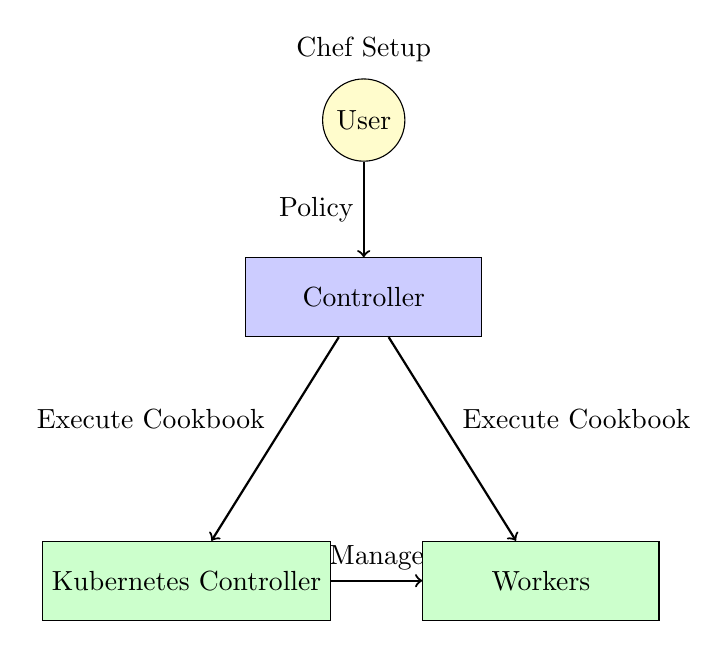
\begin{tikzpicture}[scale=0.9]
    
    % Draw the user
    \node[draw, circle, minimum size=1cm, fill=yellow!20] (user) at (0, 2.5) {User};
    
    % Draw the controller
    \node[draw, rectangle, minimum width=3cm, minimum height=1cm, fill=blue!20] (controller) at (0, 0) {Controller};
    
    % Draw the workers
    \node[draw, rectangle, minimum width=3cm, minimum height=1cm, fill=green!20] (worker1) at (-2.5, -4) {Kubernetes Controller};
    \node[draw, rectangle, minimum width=3cm, minimum height=1cm, fill=green!20] (workerN) at (2.5, -4) {Workers};
    
    % Draw connections
    \draw[->, thick] (user) -- node[midway, left] {Policy} (controller);
    \draw[->, thick] (controller) -- node[midway, above left] {Execute Cookbook} (worker1);
    \draw[->, thick] (controller) -- node[midway, above right] {Execute Cookbook} (workerN);
    \draw[->, thick] (worker1) --node[midway, above] {Manage} (workerN);
    % Optional: Add labels
    \node at (0, 3.5) {Chef Setup};
    % \node at (0, -5.5) {Executing Cookbooks};
    
    \end{tikzpicture}
    \caption{Example Chef Infrastructure}
    \label{fig:chef-infrastructure}
\end{figure}

% \subsection{Moving to a Bigger Scale}
% If the goal of the development would be 
% Local Development within an Ansible-Provisioned Machine and Migrating to the Cloud.





% Some of these were: different inventory.cfg needed for different local operating systems, some commands that could be executed locally displaying different behavior in the playbook, it being hard to update machine system configurations, limited verbosity in command outputs and very long wait times\cite{ansible-slow}. 

% At the end of the assignments, there is a complete local development environment. In this environment we can provision machines

% At the end of this project, we have a fairly complete local development environment. If this were a real-life situation, one would want to migrate the functionality we have created to an environment which a lot of people can use. 
